%!TEX root=writeup.tex
\section{Approach}
\label{sec:framework}

\begin{figure}
    \begin{center} 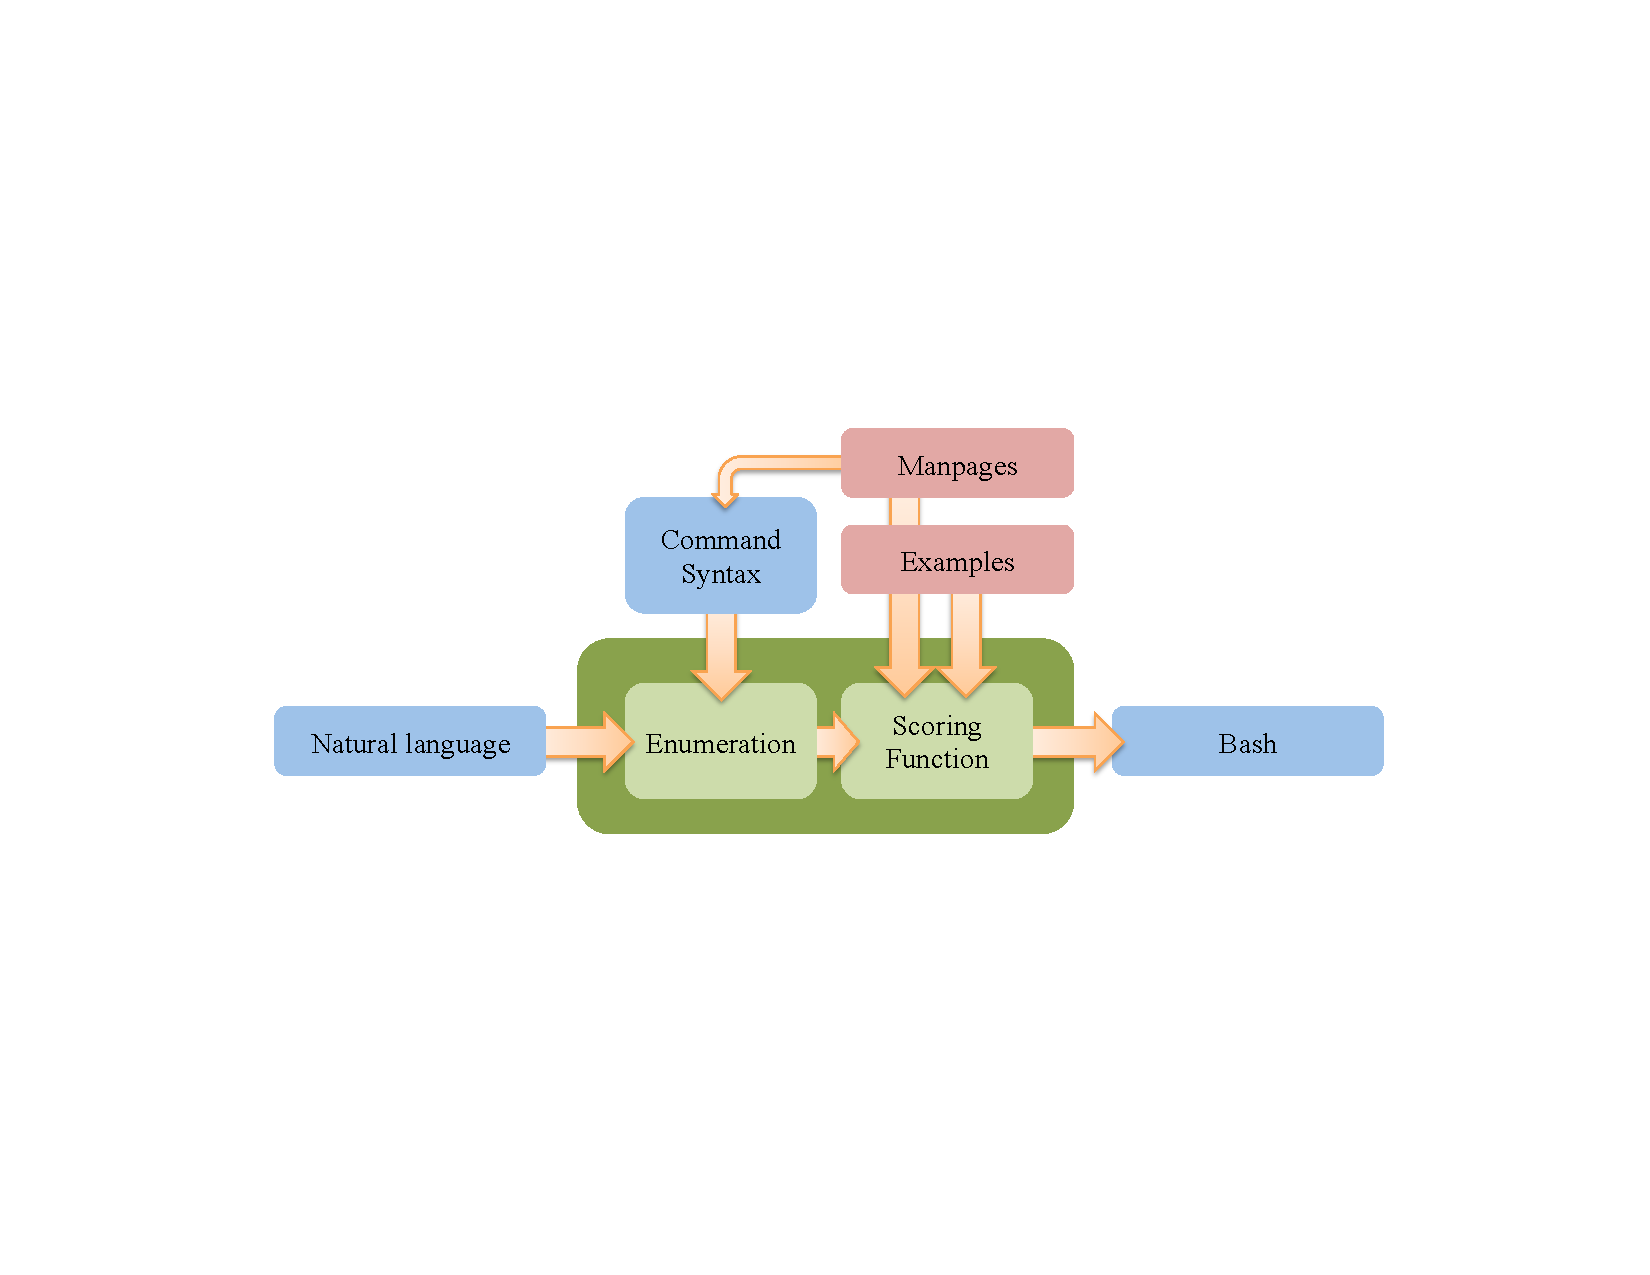
\includegraphics[width=4in]{architecture.pdf} \end{center}
    \caption{The overall architecture of our framework.}
    \label{fig:arch}
\end{figure}

\autoref{fig:arch} shows the major components of our translation framework.
Offline, the tool learns the syntax of common Bash commands using manpages. Both
the manpages and input-output examples obtained from StackOverflow are used to
learn an appropriate scoring function. At runtime, the tool enumerates possible
candidate programs using the learned syntax, scores them using the learned
scoring function, and presents the top-ranked suggestions to the user.

Section~\ref{subsec:represent} introduces the subset of Bash our tool supports
and how we obtain that subset automatically from manpages.
Section~\ref{subsec:parser} describes training and running the semantic parser.

%!TEX root=writeup.tex
\subsection{Bash Syntax and Manpage Extraction}
\label{subsec:represent}

The core Bash syntax (\autoref{fig:bash-syntax}) is very simple, but every tool imposes its own constraints on top of this. For instance, \<-c> is not a valid flag for the \<mv> tool. The translation task is much easier if these additional constraints are available at translation time. Fortunately, in this domain they do not need to be hand-coded; publicly-available manpages already document the acceptable ways to call each tool.

\begin{figure}[ht]
\begin{align*}
\mathit{bash} \quad :=& \quad \mathit{cmd} ~\mid~ \mathit{bash}|\mathit{cmd} \\
\mathit{cmd}  \quad :=& \quad \mathit{word}~(~\mathit{word}~)^{*}
\end{align*}
\vspace{-20pt}
\caption{Core bash syntax}
\label{fig:bash-syntax}
\end{figure}

%%% This paragraph is a good point, but probably not one we need to make here.
%%%   -- Calvin
% The key design tradeoff for the language is the level of declarativity. The more declarative the langauge is, it is easier to perform translation, e.g. if \code{max} is provided as a primitive of the language, it is possible to direct translate descriptions with notion of maxinum into a command using the primitive \code{max}, on the other hand, if it is not provided, the command should be achieved using \code{sort} following by \code{first} to acheive the same goal, which is less straightforward compared to the first case. However, when the language is too declarative, collecting training data are harder, as it is harder to transform real bash commands in the dataset to its intermediate representation. In our design, we choose the latter case, to make the language designed to be closer to the original bash commands, so that we can directly parse a bash command into its intermediate representation, which provides us a larger set of traning data. \autoref{fig:lang} presents the syntax of the intermediate language.

\autoref{fig:grammars} shows the kind of syntax we are able to infer from
manpages, and \autoref{fig:manpage-extraction} shows an example extraction for
the \<sort> manpage. The extracted grammars simply substitute for \|cmd| in the
overall grammar from \autoref{fig:bash-syntax}.

The extracted grammars have a very structured form. The empty string $\epsilon$
is usually used in conjunction with the cases construct to describe optional
flags, as in the case of $(\epsilon \mid \text{``-s''})$. Exact strings usually
represent flags such as \<-v> or \<-r>. The Arg form indicates that an arbitrary
string may be used; these are placeholders for arguments, such as the filename
arguments to \<rm> or \<mv>. Type information (while not used in the current
system) is generally present and may improve future iterations of our tool.
Finally, the sequence construct can chain together sequential pieces of a
grammar. Notably, we always infer a strict order among the flags for a given
command. This further restricts our output space, yielding increased performance
without impairing expressiveness.

\begin{figure}[h]
    \begin{center}
    \begin{minipage}[t]{0.4\linewidth}
        \[\begin{array}{rrll}
        G   & :=   & \epsilon                & \text{(Empty string)} \\
            & \mid & \text{``\|word|''}      & \text{(Exact string)} \\
            & \mid & \text{Arg} ~ \|type|    & \text{(Argument)} \\
            & \mid & G_1 ~ G_2 ~ ...         & \text{(Sequence)} \\
            & \mid & G_1 \mid G_2 \mid ...   & \text{(Cases)} \\
        \end{array}\]
    \end{minipage}
    \begin{minipage}[t]{0.5\linewidth}
        \[\begin{array}{rrl}
        \|type| & :=   & \text{File}
                  \mid   \text{Number}
                  \mid   \text{Pattern}
                  \mid   \text{PermissionMode} \\
                & \mid & \text{Size}
                  \mid   \text{Username}
                  \mid   \text{Groupname}
                  \mid   \text{Unknown}
        \end{array}\]
    \end{minipage}
    \end{center}
    \caption{Syntax of grammars extracted from manpages.}
    \label{fig:grammars}
\end{figure}

%%% This figure is glorious, but it is not reflective of the tool we actually
%%% built.
%%%   -- Calvin
% \begin{figure}[ht]
% \[
% \begin{array}{rlll}
% \multicolumn{3}{l}{\textbf{Program}}\\
% \mathit{p} & :=  & \mathit{cmd}~\overline{\mathit{option}} & \textrm{(Program)}\\
%     &  & \mathit{p} ~|~ \mathit{p} & \textrm{(Pipelined programs)} \\
% \mathit{option} & := & \mathit{flag} & \textrm{(Command flag)}\\
%                 &    & \mathit{val} & \textrm{(Value)}\\
% \mathit{cmd} & := & ... & \textrm{(Command names)}\\
% \mathit{flag} & := & ... & \textrm{(Flag names)}\\
% \mathit{val} & := & ...  & \textrm{(Primitive values)}\\
% ~\\
% \multicolumn{3}{l}{\textbf{Command Signature}}\\
% \mathit{sig} & := & \mathit{name}~\mathit{op} & \textrm{(Command signature)}\\
% \mathit{op} &:= & \mathit{flag} & \textrm{(Flag)}\\
%                 &   & \mathit{arg}:\tau & \textrm{(Argument)}\\
%                 &   & \mathit{arg}:\tau~...& \textrm{(Argument list)}\\
%                 &   & \mathit{op}~\mathit{op} & \textrm{(Sequential options)}\\
%                 &   & \mathit{op}~|~\mathit{op} & \textrm{(Exclusive options)}\\
%                 &   & [ \mathit{op} ] & \textrm{(Optional options)}\\
% ~\\
% \multicolumn{3}{l}{\textbf{Rules}}\\
% \mathit{rule}^{*} &:=& \mathit{cmd}~\overline{\mathit{option}} : \tau & \textrm{(Command typing rule)}\\
% ~\\
% \multicolumn{3}{l}{\textbf{Types}}\\
% \tau_0 & := & \mathsf{void},~ \mathsf{File},~ \mathsf{Date},~\mathsf{Perm} ...& \textrm{(Primitive types)}\\
% \tau & := & \tau_0 ~|~ (\bar{\tau}_0)\rightarrow \tau_0 & \textrm{(Type)}
% \end{array}
% \]
% \caption{Intermediate Language syntax, where $\mathit{cmd}$ ranges over strings presernting command names, $\mathit{flag}$ are strings presenting flag names, $\mathit{val}$ presents values in bash programs, and $\mathit{arg}$ represents meta-argument names.}
% \label{fig:lang}
% \end{figure}

% In the intermediate language, \textit{Program} defines the formation rules for a command: i.e. a command is either a primitive command or the pipeline of two programs. However, not every programs that can be represented by the syntax is valid, e.g. the program \code{find -goal} is well formed under the syntax, but it is not a valid real CLI program, as the \code{goal} flag is not part of the command \code{find}. Thus, \textit{command signatures} are introduced to check the well-formedness of a given bash command.

% \textit{Command signature} in \autoref{fig:lang} defines the usages for certain commands: a command is well formed only if it follows its corresponding structure. \textit{types} reflect the type of an argument, helping restrict usage of values in a command as types used in other typed languages. Figure~\ref{fig:cmdsig} shows the signature of some commands used in our system. With this signature, the command \code{mv -f -v a.txt b.txt} is will formed as it is captured by the signature of \code{mv}.

\begin{figure}
    \begin{center}
    \begin{minipage}[t]{0.6\linewidth}
        \textbf{Manpage:} \\
        \begin{lstlisting}[gobble=8]
        ...

        SYNOPSIS
            sort [-bdfgiMnrckmosStTuz] [file ...]

        DESCRIPTION
            ...

            -s, --stable
                   stabilize sort by disabling last-resort comparison

            -S, --buffer-size=SIZE
                   use SIZE for main memory buffer

            ...
        \end{lstlisting}
    \end{minipage}
    \begin{minipage}[t]{0.39\linewidth}
        \textbf{Extracted grammar:} \\
        \begin{align*}
            \text{``sort''} ~ ~ & ... \\
                & (\epsilon \mid \text{``-s''}) \\
                & (\epsilon \mid (\text{``-S''} ~ (\text{Arg Size}))) \\
                & ... \\
                & (\epsilon \mid (\text{Arg File}))
        \end{align*}
    \end{minipage}
    \end{center}

    \caption{Sample grammar extraction for \<sort> using the grammar syntax
        from \autoref{fig:grammars}.}
    \label{fig:manpage-extraction}
\end{figure}

Our manpage extraction looks at the \<SNYPOSIS> section of the manpage to obtain
the legal list of flags as well as the names and types of positional arguments.
The \<DESCRIPTION> section describes each flag in more detail, and from this we
obtain information about arguments to flags and their types.

%!TEX root=writeup.tex
\subsection{Natural Language to Bash Command Translation}
\label{subsec:parser}

We adopted a top-down approach that searches for the most relevant bash commands for a given natural language description. Specifically, we designed an efficient greedy search procedure (\S~\ref{subsec:decoding}) that enumerates the set of relevant bash commands generated by the bash grammar presented in \autoref{fig:grammars}, and extracts a set of features for each of them paired with the natural language description (\S~\ref{subsec:feature}). The set of candidate commands are then ranked by a linear scoring function, the weights of which are learned from a training set (\S~\ref{subsec:training}).

\subsubsection{Decoding}
\label{subsec:decoding}

To control scalability, we consider only the following small set of head commands: \texttt{find, mv, sort, grep, cp, ls, tar, xargs}. Nevertheless, the number of possible bash commands covered by this set is still daunting. Take the \texttt{find} command as an example, it has nearly 40 options and hence $2^{40}$ bash command candidates\footnote{Most of the command-option combinations are pretty rare. However, we haven't found an effective way to guide search with this information.}. To prevent the search space from blowing up, we consider only candidate commands that contain $2-5$ terms (a ``term'' is either a head command, a flag, or an argument). Furthermore, we use a greedy search procedure which only explores the top-$k$ best children of each node based on the scoring of the partial command ending at the child node. We designed the features to be factorized over each term of the program, i.e. a set of features are extracted for each term in the command candidate and the final feature set is the union of them. This allows features of a bigger program structure to be computed based on the features of its substructures. While this simplified feature set misses most information regarding both the structure of the commands and the structure of the language, we found it to frequently capture the gist of a translation in practice.

The greedy procedure for bash command enumeration and feature extraction is summarized in alg.~\ref{alg:decoding}.

\begin{algorithm} [ht]
\caption{Bash command enumeration and feature extraction\label{alg:decoding}}
\SetKwInOut{Input}{Input}
\SetKwInOut{Output}{Output}
\SetKwInOut{Initial}{Initialization}
\SetKwFunction{Add}{AddTo}
\SetKwFunction{DFS}{DFS}
\SetKwFunction{ExtractFeat}{ExtractFeatures}
\SetKwFunction{TopKBest}{TopKBestNextTerms}
\SetKwFunction{EndOfCmd}{IsEndOfCmd}
\SetKwFunction{PrintCmd}{GetCmdAndFeaturesWithBacktracking}

\Input{nl\_cmd, HeadCmdSet}
\Output{CmdsAndFeatures}
\Initial{CmdsAndFeatures=\{\}}
\For {head\_cmd $\in$ HeadCmdSet}{
	\DFS{head\_cmd, nl\_cmd}
}
\SetKwProg{fun}{Procedure}{}{}
\fun{\DFS{term, nl\_cmd}}{
	term.features = \ExtractFeat{term, nl\_cmd} \\
	\If {\EndOfCmd{term}} {
		CmdsAndFeatures $\leftarrow$ CmdsAndFeatures + \\
			\PrintCmd{term}
	}
	\For {next\_term $\in$ \TopKBest{term}} {
		next\_term.backpointer = term \\
		\DFS{next\_term, nl\_cmd}
	}
}
\fun{\ExtractFeat{term, nl\_cmd}}{
	FeatureSet = $\emptyset$

	\For {word $\in$ nl\_cmd} {
		FeatureSet = FeatureSet + (term, word)
	}
	\KwRet{FeatureSet}
}
\end{algorithm}

\subsubsection{Features}
\label{subsec:feature}
% The following features are used:
% \begin{itemize}\itemsep-1pt
%	\item association of key words/phrases to partial expressions
%  	\item association between partial expressions (e.g. how often do they combined in valid commands)
%	\item similarity of key words/phrases in the command to the man page explanation text of a partial expression
%	\item complexity of the logical formulas and the commands generated from them.
% \end{itemize}
As shown in the bottom function in alg.~\ref{alg:decoding}, the feature set consists of simple term-word tuples, where a \emph{term} is a token found in Bash source code and a \emph{word} is an English word in the natural language. When a term appears in the input that was not present in the training data, we replace it with the special ``unk\_term'' symbol. Similarly, and any unseen words become the ``unk\_word'' symbol. To discriminate important features from unimportant ones, we assigned each tuple its PMI value, which is computed on the training set using the following equations:

\begin{align}
	\|PMI|(t, w) &= \log{\frac{P^2(t,w)}{P(t)P(w)}} \\
	P(t, w) &= \frac{\|count\_of\_|(t,w)}{\|total\_count\_of\_tuples|} \\
	P(t) &= \frac{\|count\_of\_t|}{\|total\_count\_of\_terms|} \\
	P(w) &= \frac{\|count\_of\_w|}{\|total\_count\_of\_words|}.
\end{align}

The PMI value measures the association between a pair of term and word based on the training set. It has the effect of down-weighting uninformative tuples such as ``(\texttt{find}, and)''---both \<find> and ``and'' are very common tokens. However, we also noticed some anomalies associated with this approach. For example, the tuple ``(\texttt{-f}, file)'' has a very low PMI value, although the \texttt{-f} option generally refers to a file. This is because the word ``file'' occurs in almost every training example in our dataset (with and without \texttt{-f} present). Therefore simple example-level occurrence measure wasn't able to reveal the connection between \texttt{-f} and ``file''. We suspect that statistical alignment, which infers the probability of the alignment between each term and word in every example, would work better than exhaustive pair-up. The design of an alignment algorithm is left to future work.

\subsubsection{Training}
\label{subsec:training}

We use the structured perception algorithm (alg.~\ref{alg:training}) to learn weights of the scoring function from the example pairs. In the training process, the input are pairs collected from StackOverflow, and the target is to learn a scoring functions to evaluate the correspondence between the a natural language description and a bash command. In each training iteration, top ranked logical form are selected and the weights are updated based on its similarity to the ground truth logical form.

\begin{algorithm}
\caption{Perceptron Training\label{alg:training}}
\SetKwInOut{Input}{Input}
\SetKwInOut{Output}{Output}
\SetKwFunction{Feat}{FeatureVectorOf}
\SetKwFunction{TopPred}{TopPrediction}
\Input{$\{(bash\_cmd_i,nl\_cmd_i)|i=1\hdots N\}$}
\Output{weights}
\For{$t = 1,\hdots, T$}{
	\For{$i=1\hdots N$} {
		prediction = \TopPred{$nl\_cmd_i$}

		\If {prediction != $bash\_cmd_i$} {
			weights = weights + 2 * \Feat{$bash\_cmd_i$} - \Feat{prediction}
		}
	}
}
\end{algorithm}

